\documentclass[12pt,letterpaper]{scrreprt}

%----------------------------------------------------------------------
%				Required Packages
%----------------------------------------------------------------------
\usepackage{usecases}
\usepackage{enumitem}
\usepackage{graphicx}

\usepackage[top=2cm,bottom=3.5cm]{geometry}

%----------------------------------------------------------------------
%				Title Page
%----------------------------------------------------------------------
\title{CS383: Software Engineering}
\author{
			Sean Shepherd\\
			\texttt{shep1244@vandals.uidaho.edu}
			\\
			Chi-Hsiang Wang (\LaTeX\ Layout)\\
			\texttt{wang0162@vandals.uidaho.edu}								
			\\
			Cameron Simon\\
			\texttt{simo2703@vandals.uidaho.edu}					
			\\
			Joe Higley\\
			\texttt{higley@vandals.uidaho.edu}				
			\\
			Ian Westrope\\
			\texttt{west2737@vandals.uidaho.edu}
			\\
}


\date{}

%----------------------------------------------------------------------
%				Additional Settings
%----------------------------------------------------------------------
\setcounter{tocdepth}{3}
\setcounter{secnumdepth}{3}




%----------------------------------------------------------------------
%				Use Case Document Start
%----------------------------------------------------------------------
\begin{document}


\maketitle

\chapter {Scenario Class Diagram}
\begin{figure}[ht!]
\centering
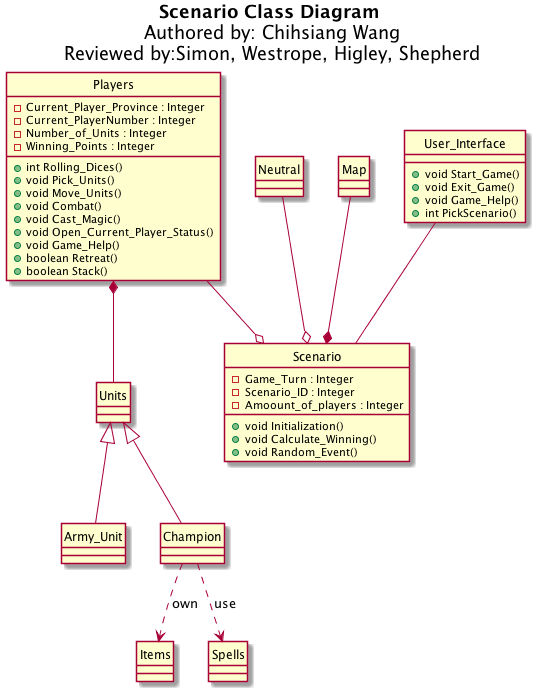
\includegraphics[width=100mm]{Scenario Class Diagram.png}

\end{figure}

I designed the Scenario class diagram, but since Scenario is the big map of this project, so I also make the overview class diagram, also include user interface class. Since it's clearly for each classes' relation, more details will be shown in other class diagrams.




\chapter {Map Class Diagram}


\begin{figure}[ht!]
\centering
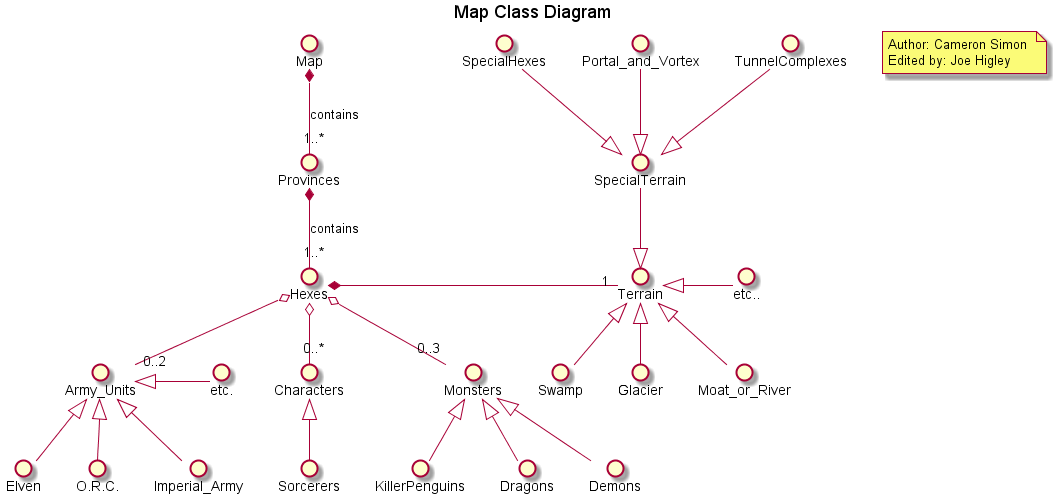
\includegraphics[width=170mm]{Map Class Diagram.png}
\label{overflow}
\end{figure}


Map Class Diagram Description\\
Author: Cameron Simon\\

Map has to be made up of at least one province (absolute aggregation).
Province made up of at least one Hex (absolute aggregation).
Hex's have to consist of at least terrain(absolute aggregation) but can 
also consist of Army Units (0..2), Characters(0..*), or Monsters(0..3).
The extensions Army Units are Elves, O.R.C.'s, Imperial Armies, etc. because
those are Army Units.
The extension of Characters is Sorcerers because Sorcerers are characters.
The extensions of Monsters are KillerPenguins, Dragons, and Demons because
those are Monsters.
The extensions of Terrain are SpecialTerrain, Swamp, Glacier, Moat or River, 
etc. because those are types of terrain.
The extensions of Special Terrain are Special Hexes, Portal and Vortex, and 
TunnelComplexes because those are types of special terrain.





\chapter {Units Class Diagram}


\begin{figure}[ht!]
\centering
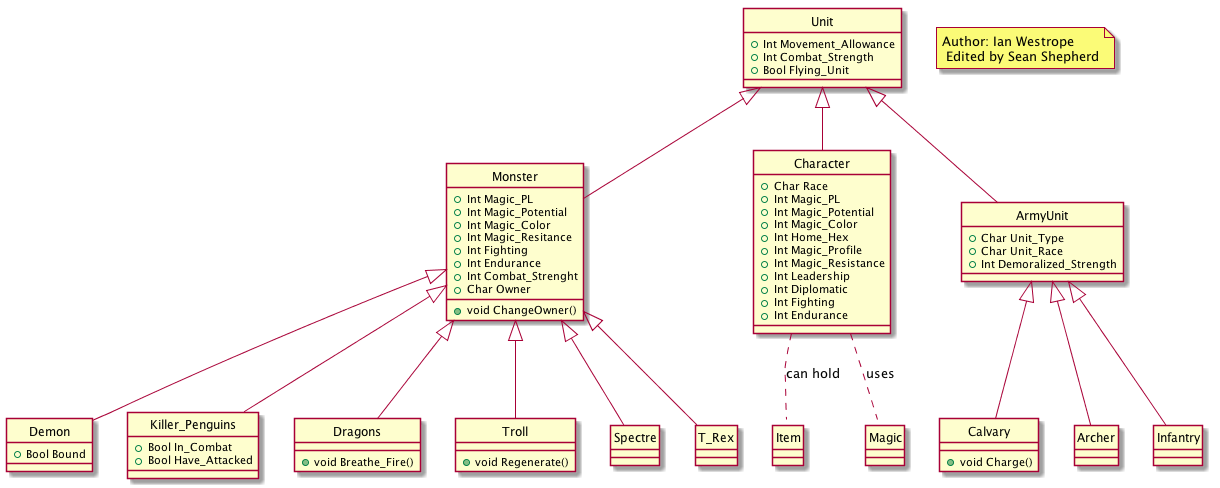
\includegraphics[width=160mm]{Units Class Diagram.png}
\label{overflow}
\end{figure}

    
The Units class diagram is generally straight forward. The only part that needs
some explaining is where a Character can hold an Item(s) or that a Character 
can cast a spell using the Magic class. Other than those two cases the rest of
the diagram is pure inheiritance between classes. 
    
    



\chapter {Items Class Diagram}


\begin{figure}[ht!]
\centering
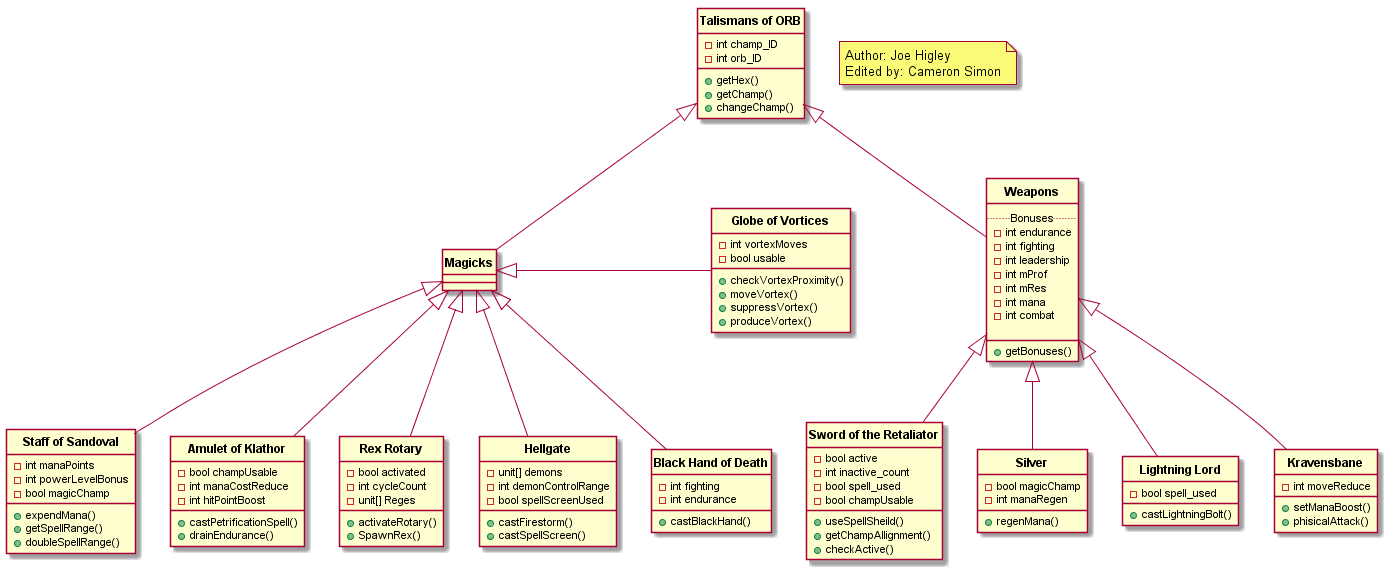
\includegraphics[width=160mm]{Item Class Diagram.png}
\label{overflow}
\end{figure}

Item Class Diagram\\
Author: Joe Higley\\

I read thru the entire rules section on Talismans of Orb.  It separated the Talismans into 2 types, Magicks and Weapons. So I made these the subclasses of my Talismans of Orbs.  I noticed that the Weapons all changed certain character attributs, so I made these all private members of the Weapons class that the weapons will all share. Then I placed all the different weapon and magical talismans as subclasses of the Weapons and Magicks classes respectively. The individual items have specific members and functions for each of them.




\end{document}
